\documentclass[a4paper, 10pt]{vanvliet_paper}
\newacronym{FAS}{fas}{forward association strength}
\newacronym{BAS}{bas}{backward association strength}
\newacronym[\glslongpluralkey={event-related potentials}]{ERP}{erp}{event-related potential}
\newacronym{EEG}{eeg}{electroencephalography}
\newacronym{MEG}{meg}{magnetoencephalography}
\newacronym{EMG}{emg}{electromyography}
\newacronym{EOG}{eog}{electro-oculogram}
\newacronym{MR}{mr}{motor related}
\newacronym{MRP}{mrp}{motor related potential}
\newacronym{RT}{rt}{response time}
\newacronym{LSA}{lsa}{latent semantic analysis}
\newacronym{JAM}{jam}{judgment of associative memory}
\newacronym{BCI}{bci}{brain--computer interface}
\newacronym{LME}{lme}{linear mixed effects}
\newacronym{REML}{reml}{restricted maximum likelihood}
\newacronym{ML}{ml}{maximum likelihood}
\newacronym{ROC}{roc}{receiver operating characteristic}
\newacronym{AUC}{auc}{area under curve}
\newacronym{ROC-AUC}{roc-auc}{receiver operating characteristic -- area under curve}
\newacronym{NS}{ns}{negative slope}
\newacronym{LCMV}{lcmv}{linearly constrained minimum variance}
\newacronym{stLCMV}{\textnormal{st}lcmv}{spatio-temporal linearly constrained minimum variance}
\newacronym[\glslongpluralkey={components of interest}]{COI}{coi}{component of interest}
\newacronym[\glslongpluralkey={regions of interest}]{ROI}{roi}{region of interest}
\newacronym[\glslongpluralkey={generators of interest}]{GOI}{goi}{generator of interest}
\newacronym{ANOVA}{anova}{analysis of variance}
\newacronym{SNR}{snr}{signal-to-noise ratio}
\newacronym{lSVM}{\textnormal{l}svm}{linear support vector machine}
\newacronym{SVM}{svm}{support vector machine}
\newacronym{AoA}{a\textnormal{o}a}{age of acquisition}
\newacronym{PCA}{pca}{principal component analysis}
\newacronym{ICA}{ica}{independent component analysis}
\newacronym{MCMC}{mcmc}{Markov chain Monte Carlo}
\newacronym{LR}{lr}{logistic regression}
\newacronym{LDA}{lda}{linear discriminant analysis}
\newacronym{FC}{fc}{Fisher criterion}
\newacronym{SOA}{soa}{stimulus onset asynchrony}
\newacronym{IIR}{iir}{infinite impulse response}
\newacronym{RVM}{rvm}{random vector model}
\newacronym{RPM}{rpm}{random permutation model}
\newacronym{HAL}{hal}{hyperspace analogue to language}
\newacronym{CAR}{car}{common average reference}
\newacronym{MTG}{mtg}{middle temporal gyrus}
\newacronym{STG}{stg}{superior temporal gyrus}
\newacronym{MTC}{mtc}{medial temporal cortex}
\newacronym{ATC}{atc}{anterior temporal cortex}
\newacronym{AG}{ag}{angular gyrus}
\newacronym{IFG}{ifg}{inferior frontal gyrus}
\newacronym{fMRI}{\textnormal{f}mri}{functional magnetic resonance imaging}
\newacronym{CSP}{csp}{common spatial patterns}
\newacronym{GMM}{gmm}{Guassian mixture model}
\newacronym{OAS}{oas}{oracle approximating shrinkage}
\newacronym{bCSP}{\textnormal{b}csp}{bi-linear common spatial patterns}
\newacronym{HOOI}{hooi}{higher-order orthogonal iteration}
\newacronym{AIC}{aic}{Akaike information criterion}
\newacronym{GLM}{glm}{general linear model}
\newacronym{LARS}{lars}{least-angle regression}
\newacronym{BOLD}{bold}{blood-oxygen level dependant}
\newacronym{SWLDA}{swlda}{step-wise linear discriminant analysis}
\newacronym{OLS}{ols}{ordinary least squares}
\newacronym{SVR}{svr}{support vector regression}
\newacronym{RANSAC}{ransac}{random sample consensus}
\newacronym{MSE}{mse}{mean squared error}
\newacronym{L-BFGS-B}{l-bfgs-b}{Limited-memory Broyden--Fletcher--Goldfarb--Shanno with box constraints}
\newacronym{PDP}{pdp}{parallel distributed processing}
\newacronym{CNN}{cnn}{convolutional neural network}
\newacronym{ReLu}{r\textnormal{e}l\textnormal{u}}{rectified linear unit}
\newacronym{MNE}{mne}{minimum norm estimate}
\newacronym{ECD}{ecd}{equivalent current dipole}

\addbibresource{reading_models.bib}

\draft
\title{A large scale computational model of word recognition and its comparison with MEG data}

\author[1*]{Marijn van Vliet}
\author[1]{Oona Rinkinen}
\author[1]{Takao Shimizu}
\author[2]{Barry Devereux}
\author[1]{Riitta Salmelin}
\affil[1]{Department of Neuroscience and Biomedical Engineering, Aalto University}
\affil[2]{School of Electronics, Electrical Engineering and Computer Science, Queen's University Belfast}
\affil[*]{Corresponding author: marijn.vanvliet@aalto.fi}

\begin{document}
\maketitle

\begin{abstract}
\end{abstract}

\section{Introduction}

What computational steps is the brain performing when it recognizes some lines on a piece of paper as a specific word?
This question has been the focus of a large number of neuroimaging studies that examine brain activity during reading.
Noninvasive measurement techniques such as \gls{EEG}\cite{Grainger2009}, \gls{MEG}\cite{Salmelin2007} and \gls{fMRI}\cite{Price2012} have provided a wealth of information about when and where changes in activity might be expected during various tasks involving orthographic processing\cite{Carreiras2014}.
However, it is rarely straightforward to translate observations of brain activity into a mechanistic understanding of the computational process being performed by the brain\cite{Poeppel2012}.

Computational models facilitate the development of cognitive theories by allowing us to reason about conceptual "box and arrow" ideas in a qualitative and quantitative manner\cite{Barber2007, Price2018}.
However, the predictions made by existing models of reading are not directly comparable to actual neuroimaging data, and it is an often repeated sentiment that there should be more contact between the two\cite{Carreiras2014, Laszlo2012, Laszlo2014, Poeppel2012, Taylor2013}.

In the domain of models of reading in the brain, connectionist models using \gls{PDP}\cite{McClelland2003} and "dual route" approaches\cite{Perry2007} have been shown to account for many observational findings in both healthy volunteers and patients\cite{McLeod2000, McClelland2003, Perry2007}.
Furthermore, \textcite{Laszlo2012} have shown that by summing the activity of the computational units in specific layers of a connectionist model, the resulting time varying signal resembles a well known component, observed in \gls{EEG} and \gls{MEG} studies, known as the N400 potential\cite{Kutas2011}.
This result has later been extended to model more of such components\cite{Laszlo2014}.
However, the signal produced by the model of \textcite{Laszlo2012} cannot be directly compared with neuroimaging data, because the simulated environment was extremely simplified to reduce the complexity of the model, whereas the brain data will by nature reflect the reading process in a realistic setting.
For example, the model operates on 5-letter words with an alphabet of only 3 possible letters.
Nevertheless, they demonstrated how a computational model can both perform a simplified reading task and produce neuroimaging-like data.

Recent advances in deep learning and its software ecosystem are rapidly changing our notion of what is computationally tractable to model\cite{Richards2019}.
\Glspl{CNN} have emerged that perform visual object recognition at a large enough scale to enable a direct comparison between network state and neuroimaging data\cite{Schrimpf2018, Devereux2018, Yamins2016} and consequently our understanding of basic visual processing has increased tremendously\cite{Lindsay2020}.
Since the first stages of reading, namely visual word recognition, can be seen as a specialized form of object recognition, \glspl{CNN} may very well be a suitable tool for increasing the scale of traditional connectionist models of reading.

In this study, we trained a \gls{CNN} to perform visual word recognition on bitmap images of rendered text.
The same set of stimulus images was presented to both the model and human volunteers in order to directly compare the activation inside the model to the amplitude of \gls{MEG} evoked responses recorded from the study participants.
Whereas the training set of the model consisted only of images of either valid Finnish words or only visual noise, the stimulus set used in the experiment contained images of valid Finnish words, which were similar to the ones present in the training data for the model, but also consonant strings, symbol strings and pseudo-words.
We show how various layers in the model behave similarly to several well studied evoked responses and evaluate this similarity both qualitatively and, for the first time, quantitatively.

\section{Results}

For the model, we used a \textsc{VGG}-11\cite{Szegedy2015} network architecture, pretrained on ImageNet\cite{Russakovsky2015}, as provided by the TorchVision package\cite{Marcel2010}.
This architecture consists of five convolution layers (three of which perform convolution twice), followed by two densely connected layers, terminating in an output layer.
The model was trained to perform visual word recognition using a training set that contained 1~000~000 images, where each image depicted one of 10~000 possible Finnish words, rendered in varying fonts, sizes and rotations, with varying degrees of visual background noise (\autoref{fig:train}).
The task for the model was to identify the correct word (by setting the corresponding unit in the output layer to a high value), irregardless of the font, size and rotation used to render the text.
The vocabulary size (10~000) was chosen to exceed the number of units in the densely connected layers (4~096) to force the model to construct a sub-lexical representation.

\begin{figure}
    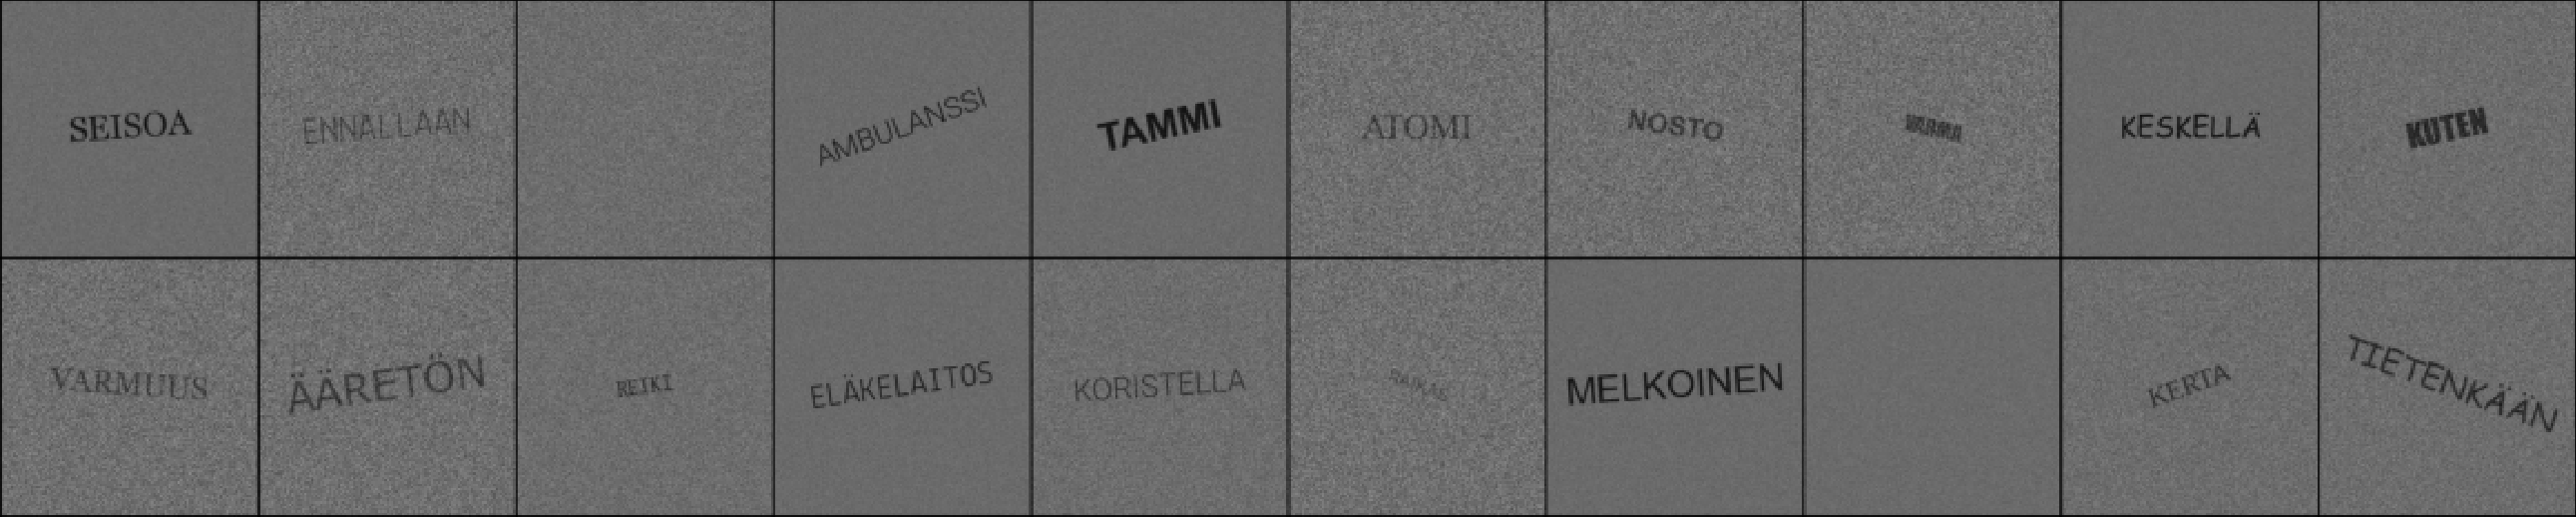
\includegraphics[width=\textwidth]{train.png}
    \caption{Examples of images in the training set for the model.}\label{fig:train}
\end{figure}

In addition to the images of valid Finnish words, 50~000 images consisting of only visual noise were added to the training set.
The inclusion of this "no word present" condition introduces a detection element to what is otherwise a discrimination task.
If no word was present in the image, all output units should have a low value.
%This was achieved by training the model with an additional output unit, indicating the "only noise" condition, while using a cross-entropy loss function, which favors only a single output having a high value, driving all other outputs to zero.
%After training, the final output unit was removed from the model.
During training, the performance of the model was evaluated on an independent test set of 100~000 images that contained words and 5~000 that contained only noise.
Training was stopped when the model's performance plateaued, at which point the accuracy on the test set was 99.3\%.

The model was compared to \gls{MEG} data that was collected as part of an earlier study by \textcite{Vartiainen2011}.
During the recording session, 15 participants were presented with various orthographic stimuli, designed to form a series of experimental contrasts that highlight three processing stages during single word reading.
The first stage is characterized by early onset activity in the visual cortex (\SIrange{65}{115}{\milli\second} after stimulus onset), which is modulated by the visual complexity of the stimulus.

% Network architecture and training
%   - Example training stimuli
%   - Test set results
% MEG experiment
%   - Previous publication
%   - Stimuli (point to figure)
%   - ECD localization (point to figure)
%   - MNE localization (point to figure)
% Big results figure
%   - Comparison of landmark behavior
%   - Statistics
\begin{figure*}
    \includegraphics[width=18cm]{results.pdf}
    \vspace{2ex}
    \caption{
        \textbf{Comparison between \gls{MEG} evoked activity and sum activity in each layer of the model.}
        Based on the response pattern to each stimulus type, three processing stages where identified that correspond to different time windows in the \gls{MEG} activity and different layer types in the model.\\
        \textbf{A)} Evoked \gls{MEG} activity, quantified during three time intervals.
        The grand-average \gls{MNE} source activity to valid Finnish words is shown in orange hues.
        Overlaid are the positions of the most representative \gls{ECD} for each participant during the indicated time interval, as determined by \textcite{Vartiainen2011}.
        Below is shown for each stimulus, the grand-average activity at the \glspl{ECD}, integrated over the indicated time interval.\\
        \textbf{B)} For each layer of the model, the sum \gls{ReLu} activation in each layer in response to each stimulus.
        The network architecture is shown below.
    }\label{fig:results}
\end{figure*}

\section{Discussion}
One may ask why the lexicon layer of the model is a one-hot encoded output vector.
This is plainly incompatible with how the brain works.
Some abstract semantic representation, such as word2vec or semantic features would clearly be better candidates.
The reason why the final layer of the model is the way it is, is because this is the point where a hard 90 degree turn needs to be made from orthographic similarity to semantic similarity.

The model used in this study is a standard convolutional design and has many shortcomings as a model of the brain.
Nevertheless, the fact that the model performs well despite these shortcomings shows the power of using deep learning models to implement cognitive theories.

\section{Methods}
\section{Acknowledgements}
We acknowledge the computational resources provided by the Aalto Science-IT project.
This research was funded by the Academy of Finland (grant \#310988 to M.v.V, \#255349, \#256459, \#283071 and \#315553 to R.S.).
% TODO: Barry funding information

\newpage
\printbibliography{}

\end{document}
